\documentclass{ou-report-vaf}

% Dit template is gemaakt door P.J. Molijn in het kader van zijn afstuderen aan de OU in 2014.
% Waarvoor hartelijk dank.
% Minieme maar belangrijke wijzigingen zijn aangebracht door E.M. van Doorn
% Het template is versimpeld door Sylvia Stuurman, 2019.
% Het template is aangepast voor de ba informatica door Harrie Passier, Tanja Vos en Pekka Aho 2020 

\usepackage[acronym]{glossaries}
\makeglossaries
\newacronym{api}{API}{application programming interface}
\newacronym{aut}{AUT}{application under test}
\newacronym{ci}{CI}{continuous integration}
\newacronym{cd}{CD}{continuous delivery}
\newacronym{cr}{CR}{capture \& replay}
\newacronym{efg}{EFG}{event flow graph}
\newacronym{eig}{EIG}{event interaction graph}
\newacronym{fsm}{FSM}{finite state machine}
\newacronym{gui}{GUI}{graphical user interface}
\newacronym{mbgt}{MBGT}{model based GUI testing}
\newacronym{mbt}{MBT}{model based testing}
\newacronym{roi}{ROI}{return on investment}
\newacronym{sut}{SUT}{system under test}
\newacronym{dbms}{DBMS}{database management system}
\newacronym{fittest}{FITTEST}{Future Internet Testing}

\begin{document}

%%%% TITLE PAGE %%%%%%%
\pagenumbering{roman} 
%to prevent that the title page will be referred as page 1, 
%which will give the warning that there is a page 1 twice.

\pagestyle{plain}
\begin{titlepage}
\begin{center}

%% Insert the OU logo at the bottom of the page.
\begin{tikzpicture}[remember picture,overlay]
    \node at (current page.south)[anchor=south,inner sep=0pt]{
        
\includegraphics[scale=0.7]{pics/OUlogo}
    };
\end{tikzpicture}

%% Extra white space at the top.
\vspace*{2\bigskipamount}

{\color{red}\Huge\bf How can model diff help the tester finding bugs}
\bigskip

{\large Research proposal}

\bigskip \bigskip
by
\bigskip \bigskip

{\Large\bf Rick Neeft}

\bigskip \bigskip\bigskip \bigskip

\begin{tabular}{lll}
%% Add additional information here, per faculty requirements, e.g
    Student number: & 851829973 \\
    Course code: & \textsc{IM}0502\\
    Thesis committee:
        & Prof. Dr. Tanja E.J. Vos (chairman), & Open University \\
        & Dr. Pekka Aho (supervisor), & Open University \\
        & Fernando Pastor Ricós (supervisor), & Universitat Politècnica de València
\end{tabular}

\end{center}
\end{titlepage}
\pagenumbering{arabic} 
%to prevent that the title page will be referred as page 1, 
%which will give the warning that there is a page 1 twice.

\let\cleardoublepage\clearpage
%%%% END TITLE PAGE %%%%%%%

%This will automatically generate your table of contents
\tableofcontents
\newpage

% Acronyms
\printglossary[type=\acronymtype]
\newpage

%%%% CONTENTS %%%%%%%

\section{Introduction}

History of GUI testing.

What role place GUI testing in the testing spectrum? (compared with unit / integration testing)

What is TESTAR?

What is a test oracle?

\newpage
\section{Background}
\subsection{How is data retrieved from the GUI}
%% give a generic introduction about the retrieval process of the GUI
%% Windows Automation API.
%% JavaAccessBridge
%% Selenium Chromedriver
\subsubsection{Windows Automation API}
\subsubsection{JavaAccessBridge}
\subsubsection{Selenium Chromedriver}

background questions. what is now and what do we already have
- what is a model? -> Background

- What are state models in TESTAR? -> background

How are state models in TESTAR Now.

\newpage

\section{Related work} \label{releatedWork}

This section contains an overview of the material that can be seen as a direct foundation for this proposal.

\subsection{Inferring state models in TESTAR}

In a recent student master graduation project, Inferring state mdoels in TESTAR, \cite{thesisMulders}  the foundation is created to build state models with TESTAR. The result can be found inside the StateModel package \footnote{\url{https://github.com/TESTARtool/TESTAR_dev/tree/master/testar/src/nl/ou/testar/StateModel}}
-> is saved in an OrientDB database - > which gives good query options -> viewer is build to see the model. 

Future work might be adding unit test on the part that will be touched since no code coverage has been found for the package.

\subsubsection{OrientDB database}

OrientDB is \textit{"the first Multi-Model Open Source NoSQL DBMS that brings together the power of graphs and the flexibility of documents into one scalable high-performance operational database."} \cite{orientdb1} 
OrientDB used Vertex and Edge classes. A Vertex is an entity that represents a node in the graph. Edge represents an entity that connects vertices. 

% add illustration about this graph.

\subsection{State model difference}
Ricós started with a proof of concept for state model difference \footnote{\url{https://github.com/TESTARtool/TESTAR\_dev/tree/state_model_difference}}
give two sut version -> calculates difference in added and removed states.

Let $A$ be a set of states of version 1 of the SUT, let $B$ be a set of states of version 2 of the SUT. The removed states can be written as
\[A-B = \lbrace x | x \in A \wedge x \notin B \rbrace\]
the states that are added can be written as
\[B-A = \lbrace x | x \in B \wedge x \notin A \rbrace\]

Future work can be viewing the SUT en all version as a universe of states to see which states are removed and added, maybe moved (if location is not part of the state)

Future work -> adding unit tests since those are not present -> refactoring of the code since some file do not have a clear Separation of concern.
\newpage

\section{Research} \label{questions}
In this section the research questions for the thesis are formulated. What is research method will be used and how the questions are being validated.

\subsection{Context}
What is the context of the research. 

\subsection{Research questions}

How can model diff help testers finding bugs???
%% specify: "What form of the answer
%% remove ambiguity
%% specify: which factors influences the RQ

- How are changes in state models detected? -> Fernando the video. no paper in TESTAR, Murphy. Image recognition might help in telling difference. 

Could it be possible to use abstract image recognition. make a screenshot of an SUT and then fill in parts, like a Text box as a rectangle, button as a solid block etc. 

% 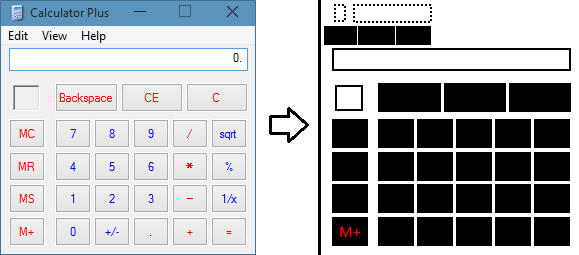
\includegraphics{document/pics/abstract-ui.png}

- What can TESTAR learn from Murphy?

- What other tools are available that uses state model difference to reason about a change? 

- How can difference in the state model become visible inside build-in state model visualisation?

- How does the build-in state model work?

sub question: How to get a useful model for the model diff.
what is a useful model... -> depends on model diff requirements

sub question- How can we tell TESTAR to ignore complete entire widgets for state abstraction?

% discusion points:
%- How can developers of GUI help in creating better models generated by TESTAR?
%- Is it bad to add testing hooks into an application? I hypothesise that adding hooks into code is not bad and can be considered a good practice when creating unit or even integration tests. Is my hypothesis correct and is it a correct hypothesis for GUI testing? I know that Microsoft provides attached properties for XAML based application (AutomationIds). Those properties are then used in code-based GUI testing.

\subsection{Research method}

\subsection{Validity}

\subsection{Planning}
\newpage

%%%%% TEMP TEXT TO TEST LATEX FUNCTIONALLY %%%%%%%%%%%%%
%%% REMOVE BEFORE PUBLISH

\section{Random things to test latex}
With a \acrshort{gui} in a \acrshort{api} you can \acrshort{aut} it with the \acrshort{cr} inside the \acrshort{ci}. To calculate the \acrshort{roi} for the \acrshort{efg} and \acrshort{eig}, it is possible to find the \acrshort{fsm}. \acrshort{mbgt} will be \acrshort{mbt} later used in the \acrshort{sut}

This is an example reference \cite{1} and \cite{2} and \cite{3} and c\cite{4}


%%%% BIBLIOGRAPHY %%%%%%%
% possible styles: apacite, abbrv, acm, alpha, apalike, ieeetr, plain, siam and unsrt.
% alpha and abbrv are most used in computer science
\bibliographystyle{alpha}
\bibliography{bibliography}

\end{document}
